\chapter{Background}
\label{Background}
\textit{Chapter starts with a general description about the \textit{\nameref{WebApplication}} structure. It is followed by a presentation of the \textit{\nameref{cia}} commonly used when discussing information security. Then follows a section about web applications \textit{\nameref{SecurityVulnerabilities}}. Finally two sections describing \textit{\nameref{DynamicTaintTracking}} and the programming language \textit{\nameref{JavaInstrumentation}}.}



\section{Web Application}
\label{WebApplication}
To make applications available and accessible from almost everywhere, companies deploy their applications on the web. The deployment of an application can vary a lot, but the most common structure for a web application is based on a three-tier architecture as illustrated in Figure \ref{fig:webApplication-Haldar}. The first tier is the presentation tier which contains the visual components rendered by the browser. Logic tier is the second part and contains the applications business logic. The third tier is the storage tier, where the business logic stores data as needed \parencite{JustinClarke-Salt2009SIAa}.
 
\begin{figure}[H]
  \centering
  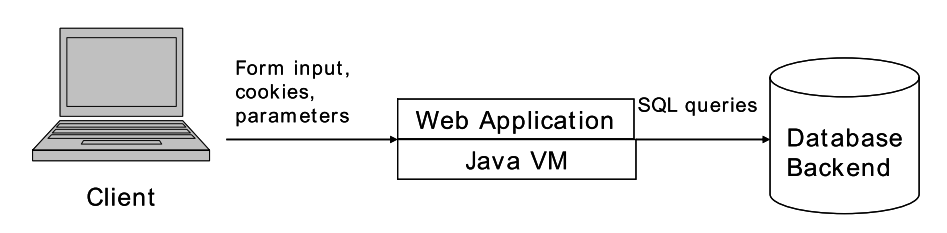
\includegraphics[width=\textwidth]{images/webApplication-Haldar.png}
  \caption{An illustration of the three-tier architecture commonly used by web applications \cite{Haldar}.}
  \label{fig:webApplication-Haldar}
\end{figure}

From Figure \ref{fig:webApplication-Haldar} it can be seen that a tier only communicates with the tier closest to themselves. This demands the logic tier to become a safeguard for the storage tier where valuable and possibly sensitive information is stored. The sensitive information might, for example, consist of username, email, personal security numbers and credit card information \parencite{JustinClarke-Salt2009SIAa}.

The scope of the thesis lies in the logic tier where both trusted and untrusted data is processed. This is the tier where validation is needed to ensure security. The programming language for the logic tier can vary a lot, but one commonly used and the chosen language for this thesis is Java \parencite{Survey}.



\subsection{Structured Query Language}
Communication between the logic and storage tier is done through a standardized language called Structured Query Language, mostly known as SQL. The SQL is created to manipulate and access databases programmatically. The majority of today's database uses SQL \parencite{Survey}. The language works by building queries specifying the required information or task. The query is then evaluated and handled by the SQL engine \parencite{DarieCristian2003TPGt}.



\section{CIA Triad}
\label{cia}
Discussions regarding information security often rely on the CIA Triad. The CIA refers to confidentiality, integrity, and availability as displayed in Figure \ref{fig:CIATriad}. Confidentiality ensures that data is only accessed by authorized individuals. Integrity specifies that application data should be accurate and unaltered. While availability is the ability to access the application and application data \parencite{2014C1-W}.

\begin{figure}[H]
    \centering
    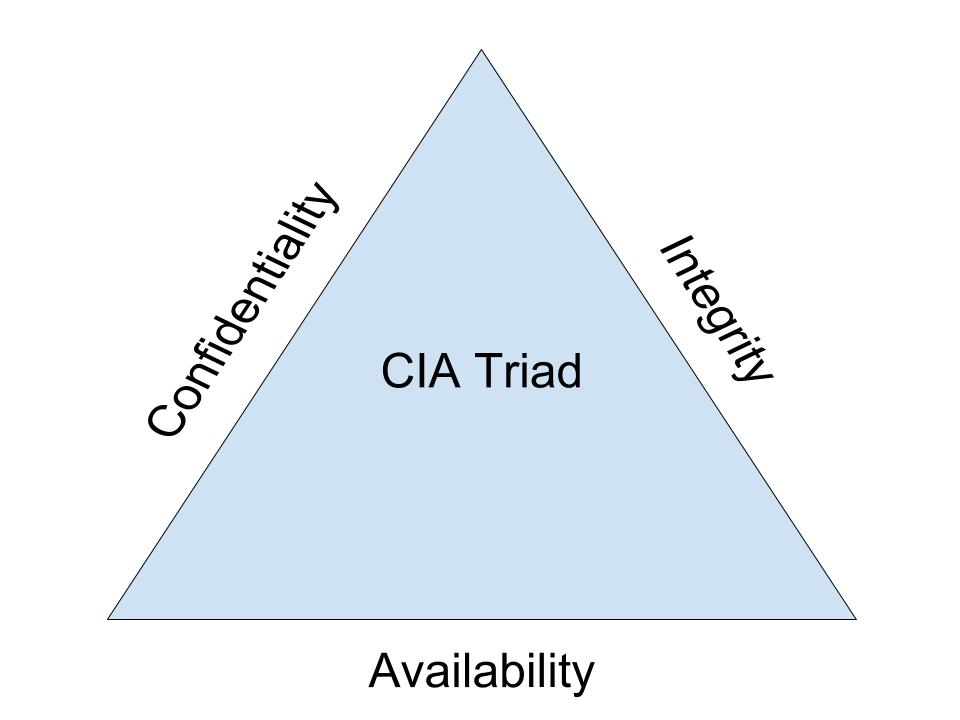
\includegraphics[height=6cm]{images/CIATriad.jpg}
    \caption{An illustration of the CIA Triad, model used when discussing information security.}
    \label{fig:CIATriad}
\end{figure}



\section{Security Vulnerabilities}
\label{SecurityVulnerabilities}
The organization Open Web Applications Security Project, known as OWASP, is an online community which aims to provide knowledge on how to secure web applications \parencite{OpenWebApplicationSecurityProject}. The OWASP has produced reports about the top ten security risks for web applications, and the latest was published in 2017. The report contains information about the ten most common security risks for the given year. Information such as how the security risk is exploited and the possible prevention methods are presented. This thesis will focus on security risk number one and seven from the mentioned report. These two security risks deal with vulnerabilities regarding information disclosure and code injection. The two vulnerabilities are Injection attack and Cross-Site Scripting \parencite{OWASP2017}.



\subsection{SQL Injection Attacks}
The most common security risk is Injection Attacks \parencite{OWASP2017}. An Injection Attack is an attack where the attacker's input changes the intent of the execution. The typical results of Injection Attacks are file destruction, lack of accountability, denial of access and data loss \parencite{Secure_Web}.

Injection attacks are executed towards a broad set of different areas, but the area discussed and analyzed in this thesis are SQL Injections. The SQL Injections can be divided into two different subgroups. These two subgroups are SQL Injection and Blind SQL Injection \parencite{Secure_Web}.



\subsubsection{SQL Injection}
The SQL Injection occurs when an SQL query is tampered with, resulting in gaining content or executing a command on the database which was not intended. Listing \ref{lst:acceptable_to_SQL_Injection} displays an SQL query which is open to SQL Injections. This due to that the variable UserId never is validated before it is propagated into the query \parencite{JustinClarke-Salt2009SIAa, Secure_Web}.

\hfill
\begin{lstlisting}[
  language=SQL,
  caption=Pseudo code acceptable to SQL Injection through malicious usage of \textit{userInput}.,
  label={lst:acceptable_to_SQL_Injection}]
userId = (*@\textit{userInput}@*)
"SELECT * FROM Users WHERE userId = " + userId
\end{lstlisting}
\hfill

The query works as intended if the user input, labeled as \textit{userInput}, is a valid Integer (since Integer is what we have decided that user id is in the application). An example of malicious usage of user input is \textit{10 or 1 = 1}. This input would result in the query seen in Listing \ref{lst:SQL_Injection}.

\hfill
\begin{lstlisting}[
  language=SQL,
  caption=An example of SQL Injection where the whole Users table is returned,
  label={lst:SQL_Injection}]
SELECT * FROM Users WHERE userId = 10 or 1 = 1
\end{lstlisting}
\hfill

This query results in an execution that always evaluates to true and therefore returns the whole table of users. This problem can be prevented in a couple of different ways. The first possibility is through validation of input, by verifying user input as in Listing \ref{lst:SQL_Injection_Verified} it is possible to protect the query from being vulnerable to a SQL Injection.

\hfill
\begin{lstlisting}[
  language=SQL,
  caption=An example of SQL Injection prevention through variable sanitiazion.,
  label={lst:SQL_Injection_Verified}]
userId = (*@\textit{userInput}@*)
isInteger(userId)
"SELECT * FROM Users WHERE userId = " + userId
\end{lstlisting}
\hfill

A second common alternative to resolve the attack is to use SQL Parameters which handle the verification for the user. This leaves the verification and validation of input up to the SQL engine. An example written with SQL Parameters can be seen in Listing \ref{lst:SQL_Injection_Parameters}.

\hfill
\begin{lstlisting}[
  language=SQL,
  caption=An example of SQL Injection prevention through SQL Parameters.,
  label={lst:SQL_Injection_Parameters}]
userId = (*@\textit{userInput}@*)
sqlQuery = "SELECT * FROM Users WHERE userId = @0"
db.Execute(sqlQuery, userId)
\end{lstlisting}



\subsubsection{Blind SQL Injection}
There also exists a blind SQL Injection which is very similar to the SQL Injection. The only difference is that the attacker does not receive the requested information in clear text from the database. The information is instead received by monitoring variables such as how long time the response takes or what kind of error messages it returns. An example of the first kind is an SQL query that tells the SQL engine to sleep depending on a condition. An example of this can be seen in Listing \ref{lst:Blind_SQL_Injection_Time} \parencite{JustinClarke-Salt2009SIAa, Secure_Web}.

\hfill
\begin{lstlisting}[
  language=SQL,
  caption=An example of Blind SQL Injection where query response is delayed five seconds if a user with id one is in the Users table.,
  label={lst:Blind_SQL_Injection_Time}]
SELECT * FROM Users WHERE userId = 1 WAITFOR DELAY '0:0:5'
\end{lstlisting}
\hfill

The second variant of a Blind SQL Injection is through analyzing error messages and, on what they return, build an image of the targeted data. This is mostly done by testing different combinations of true and false queries \parencite{JustinClarke-Salt2009SIAa, Secure_Web}.



\subsection{Cross-Site Scripting}
Another security vulnerability is Cross-Site Scripting which has been a vulnerability since the introduction of JavaScript in websites. One of the first Cross-Site Scripting attacks was carried out just after the release. The attack was conducted through loading a malicious web application into a frame on the site that the attacker wanted to gain access to. The attacker could then, through JavaScript, access any content visible or typed into the web application. The  Same-Origin Policy was therefore introduced to prevent this form of attacks. The policy restricts JavaScript to only access content from its origin \parencite{FogieSeth2007Xacs, w3csop}.

The introduction of the Same-Origin Policy, however, did not stop the attackers. The next wave of attacks was mostly directed towards chat rooms where it was possible to inject malicious Cross-Site Scripts into the message input form. This would then be reflected by the server itself, when displaying the message for other users, and thereby bypassing the Same-Origin Policy \parencite{FogieSeth2007Xacs}.

There are three different types of Cross-Site Scripting. These three are reflected, stored, and DOM-based Cross-Site Scripting.



\subsubsection{Reflected Cross-Site Scripting}
Reflected Cross-Site Scripting is mainly conducted through a malicious link that a user accesses. The malicious link will exploit a vulnerable input on the targeted web application and through the input reflect malicious content to the user \parencite{Secure_Web}.



\subsubsection{Stored Cross-Site Scripting}
Stored Cross-Site Scripting means that malicious scripts get stored in the targeted web applications database. This malicious script is then loaded and presented to each user who is trying to access the application \parencite{Secure_Web}.



\subsubsection{DOM-based Cross-Site Scripting}
DOM-based Cross-Site Scripting is very similar to Reflected Cross-Site Scripting, but it does not necessarily have to be reflected from the application server. DOM-based Cross-Site Scripting modifies the DOM tree, and through that, it exploits the user \parencite{Secure_Web}.



\section{Taint Tracking}
\label{DynamicTaintTracking}
We have now presented a set of problems that the Taint tracking, also known as taint analysis, is a tool to combat. The tool analyzes the flow of information in the application \parencite{Pan2015}. The goal of taint tracking is to prevent possible attacks such as Injection and Cross-Site Scripting by enforcing the usage of sanitizers on all untrusted input data. The Taint tracking can be implemented in two different forms: either static or dynamic. The static taint tracking is an evaluation tool possible to include in the integrated development environment where it notifies the developer of possible security vulnerabilities. The dynamic taint tracking, on the other hand, is a tool used simultaneously as the application execution. The Dynamic tracking analyses the input data to discover vulnerabilities at runtime and achieve higher accuracy compared to static tracking. The advantage with the static form is the ability to run before runtime, but its disadvantage is the lower accuracy in tracking of taint.

The Taint trackers operate by tracking untrusted data and acting upon data trying to enter sensitive code areas without first being sanitized. Perl and Ruby are two programming languages which have been adapted to use taint checking \parencite{perl, ruby}. There are some tools which enable taint checking for other platforms. One of them is TaintDroid \parencite{Ma2010} for the Android platform.

The process of taint tracking consists of four steps which are described in Table \ref{table:taintTracking}. The first step is to mark all data from untrusted sources as tainted. This is done through a taint flag attached to the variables. Step two is the possibility of detainting data, but this is only done after that the data has been sanitized through predefined sanitizers. The third step is propagating taint where tainted data propagates its tainted flag onto all data it comes in contact with. The fourth and last step is checking the taint flags in areas called sinks which are entry points to sensitive code \parencite{Pan2015, Venkataramani2008}. The decision of what to do if a tainted variable tries to pass through a sink varies depending on the application. However, remedial actions should be conducted. These actions should be, depending on the application owner´s choice, logging the events, throwing an error, or modifying the tainted values into safe predefined values. 

\begin{table}[H]
  \centering
  \caption{The four steps behind taint tracking.}
  \label{table:taintTracking}
  \begin{tabular}{rp{8.5cm}}
    \textbf{Tainting}           & Marking all data from sources as tainted.                          \\
    \textbf{Detainting}         & Marking all data from sanitizers as non-tainted.                   \\
    \textbf{Taint Propagation}     & Propagating taint to all data coming in contact with tainted data. \\
    \textbf{Assert Non-taint} & Assert that data passing through sinks are non-tainted.           
  \end{tabular}
\end{table}

An example of the taint propagation process can be seen in Listing \ref{lst:taint_propagation}. In the example \textit{getAttribute} is a source, \textit{executeQuery} is a sink and \textit{validate} is a sanitizer. On line one, the input from the source is flagged as tainted, and the taint propagates onto \textit{userId}. The sanitizer on line two validates \textit{userId} and removes the tainted flag. Lastly, the sink on line tree executes the query since the argument is not tainted. If a user sends in a malicious userId containing "101 OR 1 = 1" the validator would sanitize the String and safely execute the sink command. However, removing line two would result in tainted data entering the sink. Without a dynamic taint tracker this would result in giving the malicious user the entire list of users. With a dynamic taint tracker, on the other hand, the result is the sink halting the execution, therefore, preventing unwanted information disclosure.

\hfill
\begin{minipage}[H]{\linewidth}
\begin{lstlisting}[
  caption=A code example of accurately handling user input before accessing sensitive code area.,
  numbers=left,
  label={lst:taint_propagation}]
userId = getAttribute("userId");
validate(userId)
executeQuery("SELECT * FROM Users WHERE userId = " + userId);
\end{lstlisting}
\end{minipage}
\hfill



\section{Java}
\label{JavaInstrumentation}
Java has been a programming language in use since the early 90's. The founder's objective was to develop a new improved programming language that simplified the task for the developers but still had a familiar C/C++ syntax. \parencite{OracleVoice}. Still today Java is one of the most common programming languages \parencite{octoverse}.

Java is a statically typed language which means that no variable can be in use before being declared. The variables can be of two different types: either primitives or as references to objects. Among the primitive types does Java have support for the eight following: byte, short, int, long, float, double, boolean and char \parencite{primjav}.



\subsection{Java Virtual Machine}
There exist a plethora of implementations of the Java Virtual Machine, but the official developed by Oracle is the HotSpot \parencite{hotSpot}. One of the core ideas of Java during its development was to "write once, run anywhere." The slogan was created by Sun Microsystems which at the time was the company developing Java and the Java Virtual Machine. \parencite{Craig_2006}. The idea behind the Java Virtual Machine was to enable one language to be platform independent and then modify the Java Virtual Machine to run on as many platforms as possible. The Java Virtual Machine is a virtual machine with its own components of heap storage, stack, program counter, method area, and runtime constant pool.

Figure \ref{fig:JVM} illustrates the architecture of the Java Virtual Machine. The Class Loader loads the compiled Java code and adds it into the Java Virtual Machine Memory. The Execution Engine reads the loaded bytecode from the Java Virtual Machine Memory and executes the application instructions. The Java Virtual Machine has built-in support for Java Agents which is a tool running between the Java Virtual Machine and the executed Java application. An Agent is loaded and given access to the application by the Class Loader. The Class Loader will trigger the implemented Java Agent and allow for instrumentation of each class file loaded by the Class Loader before being loaded into the Java Virtual Machine \parencite{venners_1999, instru}.

\begin{figure}[H]
  \centering
  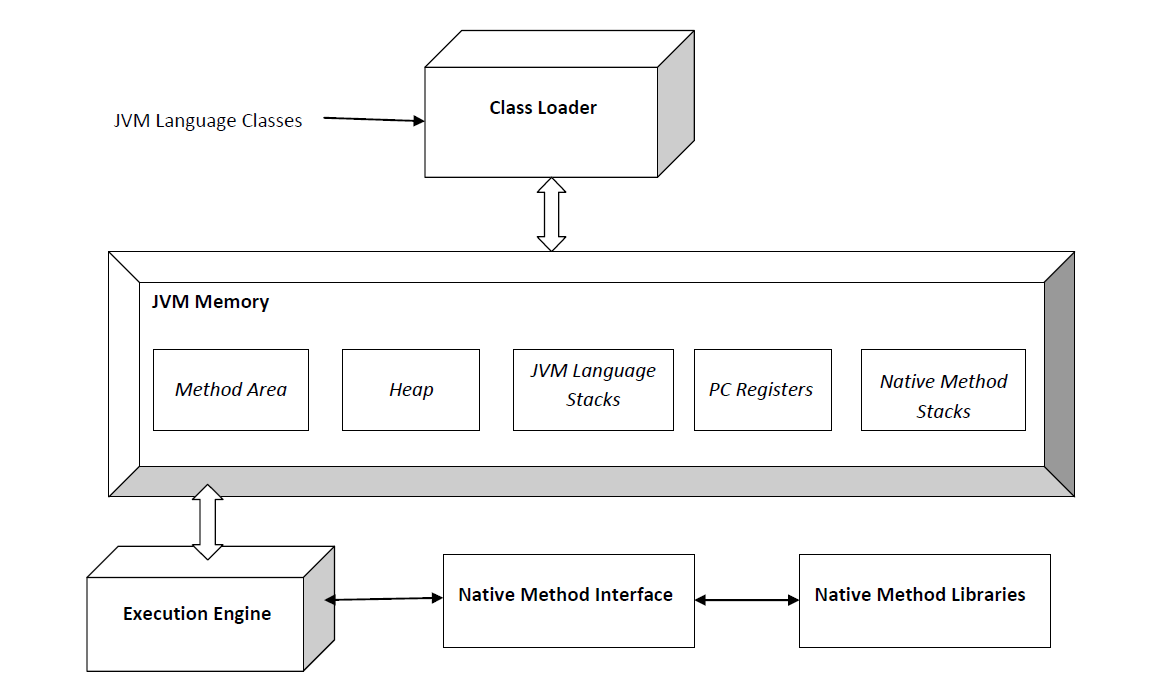
\includegraphics[width=\textwidth]{images/JvmSpec7.png}
  \caption{An illustration of the Java Virtual Machine Architecture \parencite{jvm}. }
  \label{fig:JVM}
\end{figure}


\subsection{Instrumentation}
\label{Instrumentation}
Java instrumentation is a way to modify the execution of an application without knowing or modifying the application code itself. Good use cases for Java instrumentation are, for example, monitoring agents, event loggers and taint trackers. Instrumentation is an official Java package that provides services needed to modify the bytecode of program instructions. It is conducted through implementing an Agent that makes it possible to transform every class loaded by the Class Loader before being used for the first time. However, there is a library of classes which cannot be instrumented by an Agent. This library is the rt.jar containing the Base Java Runtime Environment which is needed to start up the Java Virtual Machine including the Class Loader. The instrumentation of the Base Java Runtime Environment needs to be done before running the Java application.

The Java Agent operates on bytecode which is time-consuming work for the developer. To ease the task of instrumentation is the bytecode instrumentation library Javassist used \parencite{Java_Instrument, Javassist}.



\subsection{Javassist}
There exist several libraries that can be of help to the developer in the task of creating a Java Agent. The help comes in libraries of methods to manipulate Java bytecode. The library used in this thesis is Javassist. Javassist stands for Java Programming Assistant and provides two levels of API. The two are on source respectively bytecode level. We used the source level API which is providing the functionality of manipulating Java bytecode with little bytecode knowledge \parencite{Javassist}.

The Javassist source level API provides classes representing instances of classes, methods, and fields. These API classes contain methods to use when computing if the given class, method or field should be instrumented. The classes representing methods do also contain the methods \textit{insertBefore}, \textit{insertAfter} or \textit{insertAt}. These three methods allow inserting Java code to the beginning, the end or at a specific position of the method.
